
% Options for packages loaded elsewhere
\PassOptionsToPackage{unicode}{hyperref}
\PassOptionsToPackage{hyphens}{url}
\PassOptionsToPackage{dvipsnames,svgnames,x11names}{xcolor}
%
\documentclass[
  letterpaper,
  DIV=11,
  numbers=noendperiod]{scrartcl}

\usepackage{amsmath,amssymb}
\usepackage{iftex}
\ifPDFTeX
  \usepackage[T1]{fontenc}
  \usepackage[utf8]{inputenc}
  \usepackage{textcomp} % provide euro and other symbols
\else % if luatex or xetex
  \usepackage{unicode-math}
  \defaultfontfeatures{Scale=MatchLowercase}
  \defaultfontfeatures[\rmfamily]{Ligatures=TeX,Scale=1}
\fi
\usepackage{lmodern}
\ifPDFTeX\else  
    % xetex/luatex font selection
\fi
% Use upquote if available, for straight quotes in verbatim environments
\IfFileExists{upquote.sty}{\usepackage{upquote}}{}
\IfFileExists{microtype.sty}{% use microtype if available
  \usepackage[]{microtype}
  \UseMicrotypeSet[protrusion]{basicmath} % disable protrusion for tt fonts
}{}
\makeatletter
\@ifundefined{KOMAClassName}{% if non-KOMA class
  \IfFileExists{parskip.sty}{%
    \usepackage{parskip}
  }{% else
    \setlength{\parindent}{0pt}
    \setlength{\parskip}{6pt plus 2pt minus 1pt}}
}{% if KOMA class
  \KOMAoptions{parskip=half}}
\makeatother
\usepackage{xcolor}
\setlength{\emergencystretch}{3em} % prevent overfull lines
\setcounter{secnumdepth}{-\maxdimen} % remove section numbering
% Make \paragraph and \subparagraph free-standing
\ifx\paragraph\undefined\else
  \let\oldparagraph\paragraph
  \renewcommand{\paragraph}[1]{\oldparagraph{#1}\mbox{}}
\fi
\ifx\subparagraph\undefined\else
  \let\oldsubparagraph\subparagraph
  \renewcommand{\subparagraph}[1]{\oldsubparagraph{#1}\mbox{}}
\fi


\providecommand{\tightlist}{%
  \setlength{\itemsep}{0pt}\setlength{\parskip}{0pt}}\usepackage{longtable,booktabs,array}
\usepackage{calc} % for calculating minipage widths
% Correct order of tables after \paragraph or \subparagraph
\usepackage{etoolbox}
\makeatletter
\patchcmd\longtable{\par}{\if@noskipsec\mbox{}\fi\par}{}{}
\makeatother
% Allow footnotes in longtable head/foot
\IfFileExists{footnotehyper.sty}{\usepackage{footnotehyper}}{\usepackage{footnote}}
\makesavenoteenv{longtable}
\usepackage{graphicx}
\makeatletter
\def\maxwidth{\ifdim\Gin@nat@width>\linewidth\linewidth\else\Gin@nat@width\fi}
\def\maxheight{\ifdim\Gin@nat@height>\textheight\textheight\else\Gin@nat@height\fi}
\makeatother
% Scale images if necessary, so that they will not overflow the page
% margins by default, and it is still possible to overwrite the defaults
% using explicit options in \includegraphics[width, height, ...]{}
\setkeys{Gin}{width=\maxwidth,height=\maxheight,keepaspectratio}
% Set default figure placement to htbp
\makeatletter
\def\fps@figure{htbp}
\makeatother

\KOMAoption{captions}{tableheading}
\makeatletter
\makeatother
\makeatletter
\makeatother
\makeatletter
\@ifpackageloaded{caption}{}{\usepackage{caption}}
\AtBeginDocument{%
\ifdefined\contentsname
  \renewcommand*\contentsname{Table of contents}
\else
  \newcommand\contentsname{Table of contents}
\fi
\ifdefined\listfigurename
  \renewcommand*\listfigurename{List of Figures}
\else
  \newcommand\listfigurename{List of Figures}
\fi
\ifdefined\listtablename
  \renewcommand*\listtablename{List of Tables}
\else
  \newcommand\listtablename{List of Tables}
\fi
\ifdefined\figurename
  \renewcommand*\figurename{Figure}
\else
  \newcommand\figurename{Figure}
\fi
\ifdefined\tablename
  \renewcommand*\tablename{Table}
\else
  \newcommand\tablename{Table}
\fi
}
\@ifpackageloaded{float}{}{\usepackage{float}}
\floatstyle{ruled}
\@ifundefined{c@chapter}{\newfloat{codelisting}{h}{lop}}{\newfloat{codelisting}{h}{lop}[chapter]}
\floatname{codelisting}{Listing}
\newcommand*\listoflistings{\listof{codelisting}{List of Listings}}
\makeatother
\makeatletter
\@ifpackageloaded{caption}{}{\usepackage{caption}}
\@ifpackageloaded{subcaption}{}{\usepackage{subcaption}}
\makeatother
\makeatletter
\@ifpackageloaded{tcolorbox}{}{\usepackage[skins,breakable]{tcolorbox}}
\makeatother
\makeatletter
\@ifundefined{shadecolor}{\definecolor{shadecolor}{rgb}{.97, .97, .97}}
\makeatother
\makeatletter
\makeatother
\makeatletter
\makeatother
\ifLuaTeX
  \usepackage{selnolig}  % disable illegal ligatures
\fi
\IfFileExists{bookmark.sty}{\usepackage{bookmark}}{\usepackage{hyperref}}
\IfFileExists{xurl.sty}{\usepackage{xurl}}{} % add URL line breaks if available
\urlstyle{same} % disable monospaced font for URLs
\hypersetup{
  pdftitle={Friends\_Tvshow\_SugarbayarEnkhbayar},
  pdfauthor={Sugarbayar Enkhbayar},
  colorlinks=true,
  linkcolor={blue},
  filecolor={Maroon},
  citecolor={Blue},
  urlcolor={Blue},
  pdfcreator={LaTeX via pandoc}}

\title{Friends\_Tvshow\_SugarbayarEnkhbayar}
\author{Sugarbayar Enkhbayar}
\date{}

\begin{document}
\maketitle
\ifdefined\Shaded\renewenvironment{Shaded}{\begin{tcolorbox}[boxrule=0pt, interior hidden, frame hidden, borderline west={3pt}{0pt}{shadecolor}, enhanced, breakable, sharp corners]}{\end{tcolorbox}}\fi

\hypertarget{a-brief-description-of-the-show}{%
\subsection{1. A brief description of the
show}\label{a-brief-description-of-the-show}}

Friends is an American television sitcom created by \emph{David Crane}
and \emph{Marta Kauffman}, which aired on NBC from September 22, 1994,
to May 6, 2004, lasting ten seasons.With an ensemble cast starring
\emph{Jennifer Aniston}, \emph{Courteney Cox}, \emph{Lisa Kudrow},
\emph{Matt LeBlanc}, \emph{Matthew Perry} and \emph{David Schwimmer},
the show revolves around six friends in their 20s and early 30s who live
in Manhattan, New York City. The original executive producers were
\emph{Kevin S. Bright}, \emph{Kauffman}, and \emph{Crane}.

\emph{Kauffman} and \emph{Crane} began developing Friends under the
working title Insomnia Cafe between November and December 1993. They
presented the idea to Bright, and together they pitched a seven-page
treatment of the show to NBC. After several script rewrites and changes,
including title changes to Six of One and Friends Like Us, the series
was finally named Friends. Filming took place at Warner Bros.~Studios in
Burbank, California. The series was produced by \emph{Brightm Kauffman,
Crane} Productions and Warner Bros.~Television.

\hypertarget{a-photo-with-the-logo-or-a-shot-from-the-show-itself.}{%
\subsection{2. A photo with the logo or a shot from the show
itself.}\label{a-photo-with-the-logo-or-a-shot-from-the-show-itself.}}


\includegraphics{friends_logo.png}

\hypertarget{a-summary-of-some-basic-statistics}{%
\subsection{3. A summary of some basic
statistics}\label{a-summary-of-some-basic-statistics}}

The series finale aired on May 6, 2004, and was watched by around 52.5
million American viewers, making it the fifth-most-watched series finale
in television history and the most-watched television episode of the
2000s. The series was nominated for 62 Primetime Emmy Awards, winning
the Outstanding Comedy Series award in 2002 for its eighth season. The
show ranked no. 21 on TV Guide's 50 Greatest TV Shows of All Time and
no. 5 on Empire magazine's The 50 Greatest TV Shows of All Time. In
1997, the episode ``The One with the Prom Video'' was ranked no. 100 on
TV Guide's 100 Greatest Episodes of All-Time. In 2013, Friends ranked
no. 24 on the Writers Guild of America's 101 Best Written TV Series of
All Time, and no. 28 on TV Guide's 60 Best TV Series of All Time.

\hypertarget{a-graph-of-the-viewership-over-time}{%
\subsection{4. A graph of the viewership over
time}\label{a-graph-of-the-viewership-over-time}}

\begin{figure}

{\centering 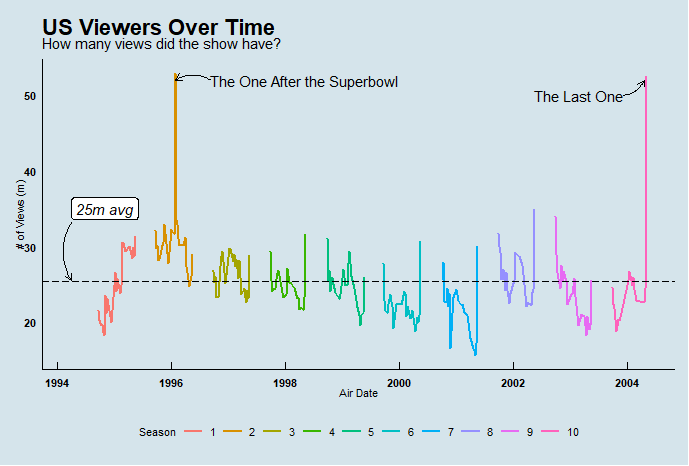
\includegraphics{friends_viewer.png}

}

\caption{Above figure shows viewership over time}

\end{figure}

\hypertarget{a-graph-of-the-episode-to-episode-or-season-to-season-changes-in-viewership}{%
\subsection{5. A graph of the episode-to-episode (or season-to-season)
changes in
viewership}\label{a-graph-of-the-episode-to-episode-or-season-to-season-changes-in-viewership}}

\begin{figure}

{\centering 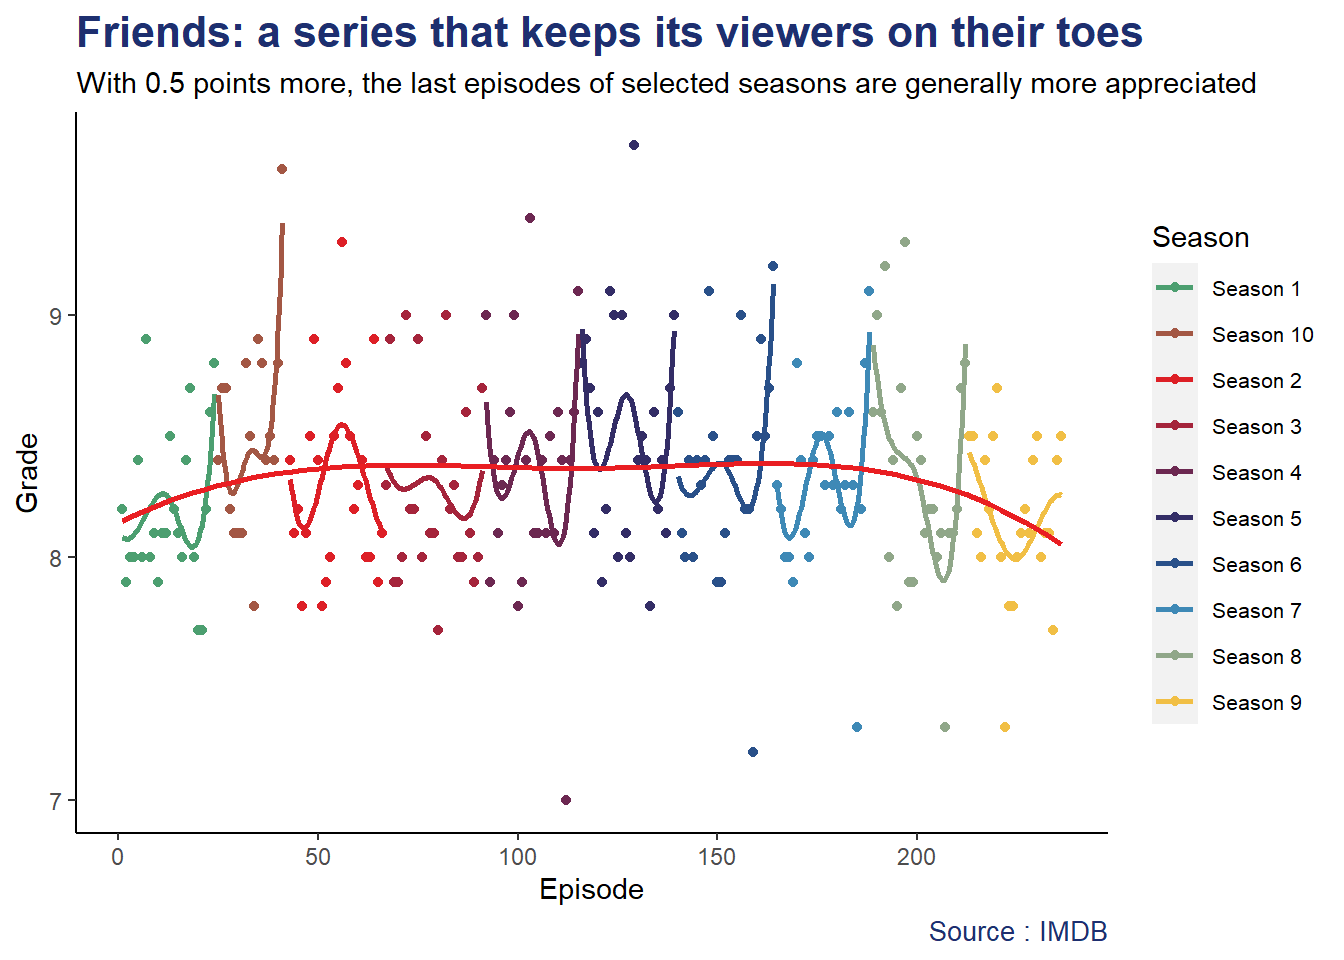
\includegraphics{friends_viewer_season.png}

}

\caption{graph shows season to season changes in viewership}

\end{figure}

\hypertarget{short-description-of-the-observed-changes-that-includes-inline-references-to-numbers}{%
\subsection{6. Short description of the observed changes that includes
inline references to
numbers}\label{short-description-of-the-observed-changes-that-includes-inline-references-to-numbers}}

viewership increased by 1 grade between seasons 1 and 10. It shows us
more people watch friends tv shows between season 1 and season 10. Each
season has average 8.5 grade.



\end{document}


